\section{研究動機}
根據雷氏(Rabiner)\cite{Rabiner}所述,
現今主導整個語音辨識研究的隱藏式馬可夫模型(Hidden Markov Model; HMM),
是在1970年代中期被首次成功地應用在語音上。
自那之後,
整體語音辨識的研究似乎受到這種新方法的刺激,
研究者們紛紛了解到統計式模型的力量,
而著手研究如何在語音辨識中適當地套用統計式方法,
因而跨入了統計式語音辨識時代。
不過,
經過長時間的研究,
至今仍鮮有能跟隱藏式馬可夫模型匹敵、
兼具辨識正確率與演算法效率等優點的模型。

延續第一個套用隱藏式馬可夫模型的語音辨識系統的架構\cite{Baker75},
現在的語音辨識系統多半是使用貝氏定理(Bayes Theorem)將語音辨識這個複雜的問題,
拆成聲學模型(Acoustic Model)及語言模型(Language Model)兩個子問題,
再分別用統計方法替兩個子問題建立模型。
早期,
研究者們在估測統計模型的參數時,
特別是訓練聲學模型時,
都是用最大相似度估測法(Maximum Likelihood Estimation; MLE)。
這個方法的目標是讓正確的轉寫(Transcription)在訓練語料中產生最大的事後機率(Posterior Probability)。
然而,
最大相似度估測法並未考慮到競爭字串(Competing Word Sequence),
導致在辨識測試語料集(Testing Set)時,
正確轉寫的聲學模型相似度(Likelihood)未必高於競爭字串的聲學模型相似度,
而造成辨識的錯誤。

直到1980年代中期,
研究者們注意到並嘗試改進這個缺點,
由當時在IBM的巴式(Bahl)\cite{Bahl}首先提出最大相互資訊估測法(Maximum Mutual Information; MMI),
開啟了往後一系列基於鑑別式訓練法則的方法。
像是最小分類錯誤估測法(Minimum Classification Error; MCE)\cite{Juang}、
最小音素錯誤模型訓練法(Minimum Phone Error; MPE)\cite{Povey}、
最小音素音框錯誤模型訓練法(Minimum Phone Frame Error; MPFE)\cite{Zheng}、
最小歧異度模型訓練法(Minimum Divergence; MD)\cite{JDu}等。
這些鑑別式訓練法則的推導方式都是基於之前的貝氏定理架構,
藉由定義不同的貝氏風險(Bayes Risk)可以得到不同的目標函數(Object Function)。
應用一些技巧最佳化上面的目標函數來得到一組新的聲學模型參數。
使用貝氏風險來考慮進鑑別觀念的好處是,
這樣不會改動原本隱藏式馬可夫模型架構,
就能獲得非常好的辨識率。

從現今的研究結果來看,
應用貝氏定理轉換建立模型的方向並拆解成兩個模型是非常成功的一步。
也就是說,
假設$Y$是所有語句、$X$是所有特徵向量序列,
貝氏定理避免我們直接為複雜的$P(Y|X)$建立模型,
而讓我們轉而替$P(Y)$、$P(X|Y)$建立模型。
並且,
使用貝氏風險導出的鑑別式訓練法則也解決了像隱藏式馬可夫模型這樣的生成模型估測參數時偏差的問題。
因此這樣看起來,
在語音辨識中採用貝氏學派(Bayesian School)的方法有極大的好處,
讓我們能輕易解決結構性輸出的問題,
這是直接為$P(Y|X)$建立模型的統計學派(Statistical School)模型在早期無法做到的。

不過機器學習領域經過這些年的發展,
一些統計學派的學習演算法逐漸發展出能應付複雜輸出(即$Y$)的改良形式。
$Y$不再受限於只有兩個類別或少數多個類別。
加上直接為$P(Y|X)$建立模型的好處是,
建立的模型多半天生就具有鑑別力,
有鑑於鑑別式訓練法則帶給語音辨識的進步,
$P(Y|X)$這樣建立模型的方向值得我們去嘗試看看。

基於以上思考,
本論文嘗試使用結構化支撐向量機(Structural Support Vector Machine; SVM-struct)直接為$P(Y|X)$建立模型,
來做基礎語音辨識的實驗。

\section{語音辨識}
為了熟悉人們前前後後嘗試過的方法,
包括何時人們從原本的方法過渡到統計式方法,
了解整個語音辨識演進的歷史是有必要的。
以下將簡介語音辨識的歷史。

根據文獻\cite{Jurafsky}記載,
第一個具有語音辨識功能的機器是一種叫雷克斯(Radio Rex)的玩具狗(見圖\ref{fig:radio_rex})。
\begin{figure}
  \centering
  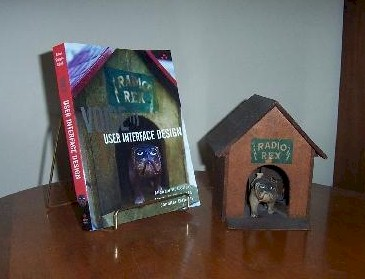
\includegraphics[scale=0.5]{images/radio_rex.jpg}
  \caption{雷克斯玩具狗} \label{fig:radio_rex}
\end{figure}
這種玩具狗在1920年代被銷售販賣,
它的賣點是,
如果有人叫他的名字「雷克斯」(Rex)的時候,
他會從底座的彈簧上彈起來。
其原理是,
玩具狗的內部有安裝一個彈簧,
這彈簧被設計成只會被500赫茲(Hz)的聲音能量驅動,
而500赫茲大約是他的英文名字Rex中第一個共振峰的頻率。

在1940年代以前,
語音辨識頂多就是像雷克斯玩具狗的共振峰辨識器一樣,
功能非常有限。
直到1940年代晚期,
才開始有一些自動化語音辨識系統被實做出來。
這邊舉兩個代表性的例子:
首先,
貝爾實驗室(Bell Lab)做了一個單一語者,可以辨識10個數字的系統。
他們的作法是在系統中存了單一語者對應十個數字的十種樣式(Patterns),
在辨識的時候就分別搜尋十種樣式,
傳回對應最高相關係數(Correlation Coefficient)的那個數字。
這樣做就可以讓系統正確率達到97\%到99\%。
第二,
在倫敦則有另一組人馬做了一個音素辨識器(Phoneme Recognizer),
它們除了採用跟前者類似的技術辨識四個母音與九個子音之外,
還率先提出音素轉移機率(Phoneme Transition Probability)的概念,
並用在他們的音素辨識器中好提昇辨識率,

到了1960年代晚期,
也是語音辨識技術革新的時期,
多數的語音辨識的技術面臨換血。
這邊列舉三個方面:

首先,
一些嶄新的抽取特徵演算法(Feature Extraction Algorithms)被提出。
包括快速傅立葉轉換(Fast Fourier Transform; FFT)、
在倒頻譜(Cepstral)空間裡處理語音訊號、
以及使用線性預測編碼(Linear Prediction Coding; LPC)來做語音編碼(Speech Coding)。

第二,
新的扭曲(Warping)技術出現。
所謂的扭曲即對訊號做時間偏移、伸展來解決說話速度(Speaking Rate)不一或訊號長度不同等問題。
扭曲一般來講都是用動態規劃(Dynamic Programming)來解決,
只是輸入的特徵向量不同而已。
舉例來講,
在早期線性預測編碼都只有用來做語音編碼。
但板倉氏結合了動態規劃的技巧與線性預測編碼。
他先對輸入的語音抽取線性預測編碼作為特徵向量,
然後對特徵向量做動態規劃來進行比對(Match)。

第三,
隱藏式馬可夫模型被應用到語音上。
隱藏式馬可夫模型是在1966年由統計學家波氏(Baum)提出\cite{BaumHMM}。
五年後,
由兩個實驗室獨立地將隱藏式馬可夫模型套用在語音上。
一個是當時在卡內基美隆(Carnegie Mellon University)唸書的貝克氏(Baker),
在讀了波式的隱藏式馬可夫模型的論文後,
將演算法應用到語音處理上。
另一個則是當時在IBM瓦特森實驗室(Watson Lab)的詹氏(Frederick Jelinek),
受到夏農(Shannon)的消息理論(Information Theory)影響而發展出跟隱藏式馬可夫模型等價的系統。
IBM的系統跟Baker的系統基本上一樣,
唯獨解碼演算法(Decoding Algorithm)不同。
Baker的系統使用維特比(Viterbi)解碼演算法,
而IBM則使用堆疊(Stack)解碼演算法。

之後的20年,
由於美國國防部陸續生出了許多語音辨識方面的計畫。
像是Resource Management, Wall Street Journal Air Traffic Information System, Broadcast News, CALLHOME等等。
藉由這些計畫的交流
隱藏式馬可夫模型也因此在研究社群中廣泛地被接受。
也因為它簡潔有效率,又有高正確率的優點,
至今仍鮮有方法可以撼動它的地位。

從以上簡述的歷史可以知道,
隱藏式馬可夫模型極其重要。
因此,
以下將簡述現今被普遍使用在語音辨識的貝氏定理架構,
隱藏式馬可夫模型便是建築在此架構上。
下一章我們再詳細說明隱藏式馬可夫模型。

如果我們把語音辨識想做是給定一串訊號,
找出一個句子它唸起來最像這串訊號。
在機率模型的架構下我們可以用條件機率來表示。
假設$x$是給定的觀測語句(Observation),
也就是處理訊號過後產生的特徵向量序列(Feature Vector Sequence),
$X$是所有可能的觀測語句。
則要從所有文句$Y$中找出機率最大的文句$y^{*}$可表示成
\begin{equation}
  y^{*} = \arg \max_{y \in Y} P(y | x)
\end{equation}
其中$y$為所有文句$Y$中的某一句,
$P(y | x)$代表在$x$發生時,文句$y$的事後機率。

剩下的問題就是,
我們要如何對$P(Y | X)$建立機率模型。
以上說起來很簡單,
但實際上由於語音辨識本身的複雜度,
對於$P(Y | X)$直接建立模型是有困難度的。
於是我們就用貝氏定理(Bayes Theorem)來轉換建模方向。
\begin{equation}
  \begin{split}
    y^{*} 
    &= \arg \max_{y \in Y} P(y | x) \\
    &= \arg \max_{y \in Y} \frac{ P(x | y) P(y) }{ P(x) } \\
  \end{split}
\end{equation}
由於我們在辨識的時候都是一句一句,
所以分母的$P(x)$在辨識一個句子的時候並不重要,
因此可以重寫成:
\begin{equation}
  \begin{split}
    y^{*} 
    &= \arg \max_{y \in Y} P(y | x) \\
    &= \arg \max_{y \in Y} P(x | y) P(y) \\
  \end{split}
\end{equation}
因此,
語音辨識的問題便被拆成如何替$P(X | Y)$及$P(Y)$建立模型。
其中$P(X | Y)$可以看作是,
給定一個句子的情況下,
唸出來的訊號是$X$的機率分佈。
而$P(Y)$則可以看成,
出現句子$Y$的機率分佈。
它們對應的稱呼便是聲學模型(Acoustic Model)及語言模型(Language Model),
也符合它們實際的意義。。

如研究動機一節所述,
本論文不沿用隱藏式馬可夫模型所使用的貝氏機率架構。
而是直接替$P(Y|X)$建立模型。
為了簡化起見,
$Y$只建立到音素辨識一層而非語言辨識一層。
而作為基礎實驗的隱藏式馬可夫模型,
也就沒有使用語言模型的分數,
而是做無設限之音素辨識(Free-Phone Decoding)。

\section{相關研究}
  語音辨識的聲學模型這一塊,
  現今大多數研究傾向在隱藏式馬可夫模型為主體的架構下抽換掉某些模型元件(Component),
  試試看辨識結果是否會進步。
  包括更換掉作為隱藏式馬可夫模型輸入的特徵
  (如使用類神經網路輸出的音框上音素的事後機率\cite{HermanskyTandem}、
  使用條件隨機域輸出的音框上音素的事後機率\cite{FoslerCrandem}),
  或更改目標函數(最小分類錯誤估測法\cite{Juang}、最小音素錯誤模型訓練法\cite{Povey})等。

  但最近這幾年仍有嘗試直接去為$P(Y|X)$建立模型的研究,
  像是隱藏式條件隨機域(Hidden Conditional Random Field; HCRF) \cite{AlexHCRF, SungHCRF},
  或是條件隨機域使用多層感知器(Multi-Layered Perceptron; MLP)的事後機率當作輸入\cite{MorrisCRF}等等。
  
  至於本論文使用的結構化支撐向量機(Structural Support Vector Machine)\cite{SVMstruct}的相關研究,
  有本論文主要依據的用結構化支撐向量機來做標籤序列(Sequence  Tagging)\cite{Altun03hiddenmarkov},
  (這也是結構化支撐向量機模型剛發展時率先的應用)
  也有將結構化支撐向量機拿來作資訊檢索\cite{JoachimsSVMperf, YisongSVMMAP}。
  由於結構化支撐向量機模型參數最佳化的困難,
  也有提出更好的最佳化演算法的論文\cite{JoachimsLinearSVM}。
  甚至有研究者注意到條件隨機域與結構化支撐向量機模型結構的相似性,
  寫了技術論文比較條件隨機域與結構化支撐向量機\cite{CRFvsSVMstruct} 。
  語音方面則還沒有人探討如何應用。

\section{本論文主要的研究方法及成果}
  本論文主要探討結構化支撐向量機學習演算法是否適合拿來解決語音辨識這個問題。
  由於模型結構的複雜性,
  先嘗試使用TIMIT這套語料來做問題相對單純的音素辨識。
  實驗結果發現,
  結構化支撐向量機學習演算法在直接使用傳統特徵向量像是梅爾倒頻譜係數(Mel-Frequency Cepstral Coefficient; MFCC)、
  感知線性預測係數(Perceptron Linear Prediction; PLP)時效果不太好,
  但如果仿照串接式系統(Tandem)的模式,
  先利用多層感知器將特徵向量轉換成音素在音框上的事後機率(Posterior Probability),
  再餵進結構化支撐向量機學習演算法的時候,
  絕對的辨識正確率卻可以贏過串接式系統約1\%。

\section{章節安排}
  本論文第二章將介紹基礎實驗中使用的隱藏式馬可夫聲學模型,以及串接式系統。
  第三章將介紹支撐向量機,
  由於結構化支撐向量機的概念是基於支撐向量機,
  全面了解支撐向量機演算法的話對於理解結構化支撐向量機十分有幫助。
  所以第三章從支撐向量機設計的理念到最佳化(Optimization)演算法給予完整的推導。
  第四章將介紹結構化支撐向量機,
  介紹該模型不同於其他模型的關鍵,
  並說明用來估測結構化支撐向量機模型參數的逼近演算法。
  第五章將介紹實驗環境、
  完整的實驗流程及結果呈現並進行分析。
  第六章會提出總結以及未來展望。
